\section{\Mimir\ Architecture}

\Mimir\ is divided into a number of related modules.

\begin{description}
\item[mimir-core] The core Java library to create a \Mimir\ index on disk, add
GATE documents to the index, and then query the index once it has been built.
Also provides some abstract helper classes for the annotation storage layer,
but not the actual storage implementations (which are provided by separate
plugins, leveraging the CREOLE plugin framework of GATE Embedded).

\item[plugins/db-h2] The default annotation storage implementation.  This
stores annotation data using H2\footnote{\url{http://h2database.com}}, an
in-process embedded SQL database.

\item[plugins/sparql] A helper that can be layered on top of any other storage
implementation to provide semantic querying against a separate knowledge base,
accessible at a SPARQL endpoint.

\item[plugins/measurements] A special-purpose helper for Measurement
annotations created by the GATE {\tt Tagger\_Measurements} plugin.  Queries are
normalised into SI units so can retrieve annotations that express the same
measurement in different terms (e.g. an annotation for ``90 seconds'' would
match a query for ``1 to 2 minutes'').

\item[mimir-connector] Java library to allow indexing of GATE documents into
a \Mimir{} index.

\item[mimir-client] The client side of the \Mimir\ remote protocol, to support
distributed querying.

\item[webapp/mimir-web] A Grails\footnote{\url{http://grails.org}} plugin providing
both the user interface to create and query indexes over the web, and also the
server side of the remote protocol to expose several distributed \Mimir\
indexes as a single {\em federated} index for clients.  This is provided as a
plugin rather than an application to make it more easily customisable.

\item[webapp/mimir-cloud] An example Grails application, that uses the {\tt mimir-web}
plugin and also includes security support. This is the exact implementation used
for \Mimir{} servers supplied on the GATE Cloud
platform\footnote{\url{https://cloud.gate.ac.uk}: a platform for running GATE-based
processes on the cloud.}. This application should be suitable without any
modifications for most users.
\end{description}

\section{Building and Running a \Mimir{} Web
Application}\label{sec:building}

The {\tt mimir-core} Java library provides support for indexes that are
represented as an on-disk directory -- named {\em Local Indexes} in the rest of
this document (see the discussion about index types in
Section~\ref{sec:admin:index-types}). To get the full functionality of \Mimir{}
(including support for {\em Remote} and {\em Federated} indexes, as well as user
interfaces for system administration and searching indexes) you will need to
build and run a web application. All the web elements of \Mimir{} are
implemented as the {\tt mimir-web} Grails plugin, which can easily be included
in any Grails-based web application. The standard \Mimir{} distribution provides
such a web application, named {\tt mimir-cloud}.

\subsection{The {\tt mimir-cloud} Web Application}
\label{sec:mimir-cloud}
The {\tt mimir-cloud} web application is the actual version of the \Mimir\
software that is used on the GATECloud platform. As such, it is configured for
that particular usage scenario, where indexes have two different URLs (depending
on whether they are accessed from within the same cloud region or not), and
where the local configuration page is not made available to the user. However,
some of this behaviour is switched off when the application detects that it is
not running on the cloud, to allow it to be used as a general purpose
\Mimir{}-enabled web application.

In addition to the {\tt mimir-web} plugin, it also includes some basic support
for user authentication (using the Spring Security Grails plugin), and support
for packaging and downloading local indexes. This is probably a suitable choice
if you just need a stand-alone web application with \Mimir{} functionality, and
you do not intend to develop your own security solution.

If you are an experienced Grails developer and you intend to add your own
security solution, then you should use the {\tt mimir-web} Grails plugin
directly in your own application, as described in
Section~\ref{sec:extend:customapp}.

While we include this application as an example of a fully-fledged Grails
application using the {\tt mimir-web} plugin, you may need to modify it slightly
to make it mode suitable to your actual usage scenario.

\subsection{Binary Distribution}

Starting with version 6.0, a pre-built WAR of {\tt mimir-cloud} is available
for download from
\url{https://github.com/GateNLP/mimir/releases}\footnote{Earlier versions back
to 5.2 are available from \url{https://sourceforge.net/projects/gate/files/}}.
This can be run using any standard Java servlet container, such as Tomcat or
Jetty.  WAR files for nightly snapshot builds can be downloaded from
\url{http://jenkins.gate.ac.uk/job/Mimir/}.

\subsection{Prerequisites}

To build your own \Mimir\ web application you will need:
\begin{itemize}
\item A Java 8 or later JDK.  \Mimir\ has been tested with the Sun/Oracle and OpenJDK
  JVMs on Linux and Mac OS X.
\item Apache Maven 3.3 or later
\end{itemize}

While not strictly a pre-requisite, \Mimir\ performs much better on 64-bit
systems than on 32-bit ones, partly due to simply being able to assign more
memory to the process, but also because the larger address space allows MG4J to
memory-map many of the files that make up the index.

To run a local instance of \Mimir\ you can use the standard \cmd{./grailsw
run-app} command, but to deploy a production instance you will need a
separate servlet container such as Tomcat.

\subsection{Building}

Building \Mimir\ is a two step process.  The core Java library, remote connector
and plugins are built using Maven, the web components (which depend on the core)
are built using Grails 3.3 via the included wrapper script -- you do not need
a separate installation of Gradle or Grails.

There is a top-level Maven pom file to build all the core components, you can
run this with the standard \cmd{mvn install} command.  Once the core components
are built you can run the {\tt mimir-cloud} web application using
\cmd{./grailsw run-app} in the mimir-cloud directory.

The next step is to configure the {\tt mimir-cloud} web application, and is
described in the following section.

\subsection{Configuring}\label{sec:admin:config}

When the \Mimir\ Grails plugin is installed into a Grails application, the
\cmd{./grailsw mimir-config} command adds a base set of configuration
options to the application's {\tt grails-app/conf/application.groovy}.
This file contains a number of settings that affect the running of the \Mimir\
components. In many cases the default options will be sufficient, but you should
nevertheless check the configuration and make sure it is appropriate for your
needs.

You can modify the {\tt application.groovy} file directly, or you can use the
``external configuration'' mechanism in Grails to override these settings at
runtime in a separate {\tt application.groovy} in the working directory.

\begin{lstlisting}
gate {
  mimir {
    plugins {
      h2 {
        group = "uk.ac.gate.mimir"
        artifact = "mimir-plugin-dbh2"
      }
      myCustomPlugin = "file:/data/mimir/plugins/myCustomPlugin"
    }
  }
}
\end{lstlisting}

\Mimir\ uses the GATE plugin mechanism to allow different annotation helpers to
be added dynamically at runtime.  This section of the configuration specifies
which plugins should be loaded when the web application starts up, and
determines the kinds of annotation helpers you will be able to use in your
indexes.  You generally need at least  the standard {\tt db-h2} plugin to be
able to do anything useful with \Mimir, and you may want the {\tt measurements}
plugin as well if you will be searching on Measurement annotations and/or the
{\tt sparql} plugin if you have an external knowledge base. 
Section~\ref{sec:indexing:helpers} has more information about the standard
annotation helpers, and section~\ref{sec:extend:helpers} discusses how to
implement your own custom ones.

Plugins can be specified in one of three ways:
\begin{itemize}
\item as a set of Maven co-ordinates ``group'', ``artifact'' and an optional
  ``version'', which will load the plugin from Maven repositories in the
  normal way.  If ``version'' is omitted it defaults to the version of the
  {\tt mimir-web} plugin, so the plugin versions that match this build of
  \Mimir{}.  The standard plugins are listed (commented out) in the sample
  configuration created by {\tt mimir-config}, uncomment the ones you need.
\item as an absolute URL string (the {\tt myCustomPlugin} example above),
  which will load a directory-based GATE plugin from the given location.
\item as a relative path string, which will be resolved against the web
  application root to form a URL which is then loaded as a directory-based
  plugin.
\end{itemize}

Maven-style plugins are typically resolved at runtime by downloading from
repositories over the network, but {\tt mimir-web} provides a utility to cache
the plugins that are referenced by a configuration, along with their transitive
dependencies, so they can be loaded from within the web application rather than
downloaded from the internet (this is useful if, for example, your \Mimir\ is
running inside a locked-down firewall and cannot make outgoing web
connections).  To do this, once you have configured your plugins but before you
build your WAR file, run {\tt ./grailsw run-command cache-mimir-plugins} in
your {\tt mimir-cloud} directory.  This will create a cache in {\tt
src/main/webapp} which will be bundled into your WAR file when you build it.

\begin{lstlisting}
// ...
queryTokeniserGapp = 
    "file:/path/to/query-tokeniser.xgapp"
\end{lstlisting}

Whereas GATE's usual data model deals with annotations in terms of their {\em
character} offsets from the start of the document, \Mimir\ deals in terms of
{\em tokens}.  Queries for plain text strings in \Mimir\ must be tokenised
before they can be matched against the index, and the tokenisation applied to
the queries must match that applied to the documents that have been indexed.
The \Mimir\ Grails plugin uses a saved GATE application state (gapp file) to
perform query tokenisation, the location of which is specified here.  By default,
\Mimir\ uses the standard ANNIE English tokeniser with its default parameters.

If your tokenisation requirements are more complex, you can provide your own
saved application that will produce annotations of type Token in the default
annotation set.  To bundle your tokeniser gapp inside the WAR file, put it
under {\tt src/main/resources} and use a ``classpath:'' URL, i.e. if your
saved application is {\tt src/main/resources/custom-tokeniser.xgapp} then set
the {\tt queryTokeniserGapp} parameter to {\tt classpath:custom-tokeniser.xgapp}

\subsection{Running}

The easiest way to run the \Mimir\ cloud web app is to use the normal Grails
commands \cmd{./grailsw run-app}.  However, for performance, it is preferable
to create a WAR file using \cmd{./gradlew assemble} and run from that (using a
tool such as \htlink{http://mvnrepository.com/artifact/com.github.jsimone/webapp-runner}{webapp-runner})
For anything more than the smallest toy index it is advisable to increase the
memory available to \Mimir\ by using the {\tt -Xmx} option to your
webapp-runner command.

For production deployments, a better option is to deploy the WAR file
to a standalone servlet container such as Apache Tomcat.  If you are using
Ubuntu or Debian GNU/Linux, it is better to download the standard Tomcat ZIP
package from Apache and use that rather than installing the Tomcat available
through {\tt apt-get} as the latter is configured by default with a security
manager that interferes with \Mimir.

When deployed to a servlet container the web application reads configuration
at runtime in the standard Grails way, looking for files named
{\tt application.yml} or {\tt application.groovy} in the working directory
of the servlet container's Java process.  Any options specified in these
files override the defaults from the {\tt application.groovy} inside the WAR.

%%%%%%%%%%%%%%%%%%%%%%%%%%%%%%%%%%%%%%%%%%%%%%%%%%%%%%%%%%%%%%%%%%%%%%%%%%%%%%
\section{Upgrading from earlier versions of \Mimir}\label{sec:admin:upgrade}

Where possible \Mimir\ tries to remain compatible with indexes and databases
created by earlier versions of the software.  Where this is not possible (e.g.
due to changes in the on-disk format between versions, or revisions of the
underlying libraries that cause binary incompatibility), a facility is provided
to ``upgrade'' existing indexes to the latest format.  If you attempt to use an
old-format index in a new version of \Mimir\ the index will show in the web
interface as ``failed'', but if you click the ``details'' button on the index
information page you will see a link offering to upgrade the index to the
latest version. The upgrade process is reasonably robust but {\bf it is very
strongly recommended to back up all the index files on disk before attempting
to upgrade}.

Depending on the size of the index the upgrade process may take some time, when
it completes the index will revert to the ``ready'' state and will then be
available for searching or further indexing as normal.

%%%%%%%%%%%%%%%%%%%%%%%%%%%%%%%%%%%%%%%%%%%%%%%%%%%%%%%%%%%%%%%%%%%%%%%%%%%%%%
\section{Indexes in \Mimir}

\subsection{Types of Index}\label{sec:admin:index-types}

A single instance of \Mimir\ can host several indexes.  \Mimir\ supports
{\em local} indexes, stored in the file system of the \Mimir\ server, and
{\em remote} indexes, which are a view of an index hosted in another \Mimir\
instance (possibly on a different machine).  Several indexes (of any type) can
be combined into a {\em federated} index, which presents the group of indexes as
a single virtual index.  All the indexing and searching functionality of
\Mimir\ applies equally to all three index types.

Each \Mimir\ index has a {\em state}, and the operations that can be performed
on the index depend on which state it is currently in. Indexes spend most of
their time in the {\em ready} state, when they can index new documents and
answer queries. During various operations they may temporarilly be in a
different state, such as {\em closing} while the index is being shut down,
typically because the \Mimir{} server is itself being shut down. Sometimes a
local index is {\em failed}, indicating a problem with the index.  Typically a
failed index will need to be deleted by the administrator, though it may be
possible to recover most of the data using the index repair tool (see
section~\ref{sec:tools:repair}).

Remote indexes inherit their state from the remote server, and federated indexes
inherit their state by combining the states of their component indexes.
A federated index may occasionally appear in the {\em working} state if its
component indexes are not all in the same state, but the working state will
usually resolve to a normal state once the component indexes have synchronised.


A typical setup for a large-scale indexing task would be to have a number of
identical ``slave'' servers running \Mimir, each with a single local index.  A
single ``master'' \Mimir\ instance could then have one remote index definition
pointing to each of the slaves, and a single federated index combining the
remote indexes.  This federated index would be the point of entry into the
system and would share out indexing jobs (round-robin among the slaves) or
search requests (to all the slaves in parallel) as appropriate.

\subsection{Creating a Local Index}

Indexes in \Mimir\ are managed through the web interface.  The front page of a
newly-installed \Mimir\ is shown in Figure~\ref{fig:front-page}.
%
\begin{figure}[htb!]
\begin{center}
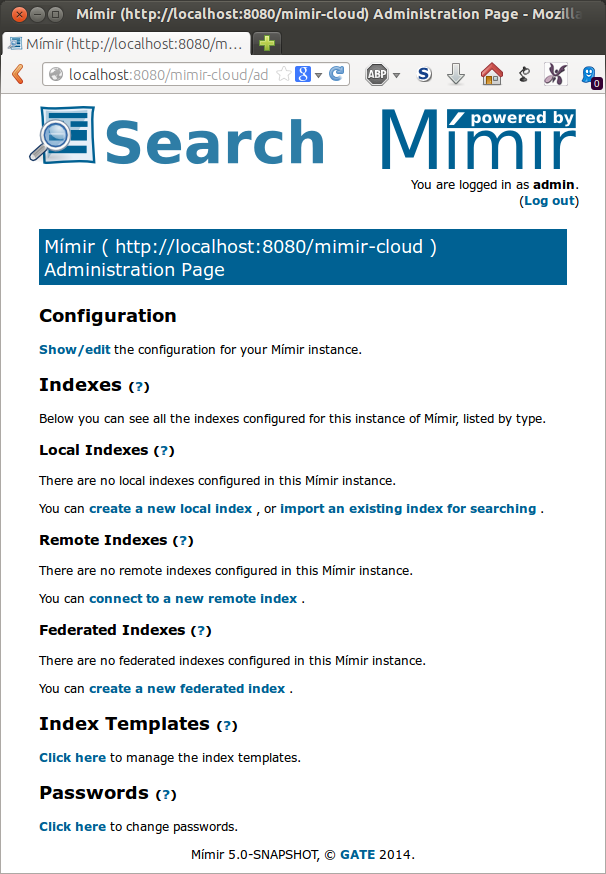
\includegraphics[scale=0.5]{img/default-front-page}
\end{center}
\caption{The default front page of a new \Mimir}
\label{fig:front-page}
\end{figure}
%
The {\em index templates} mentioned at the bottom, are used to define the
properties of new indexes, and are described in more detail in
Chapter~\ref{sec:indexing}.  The \Mimir\ Grails plugin provides a single
example template based on ANNIE annotation types.

To create an empty local index ready to receive documents for indexing, select
the {\em create a new local index} link.  This will present a form
(Figure~\ref{fig:new-local-index}) asking for the name of the new index and the
template from which it should be created.  The ``Document URIs are external
links'' option affects the way documents are presented in the search interface.
Every document in \Mimir\ is identified by a URI, and if you intend to use
document URIs that are actually resolvable URLs (for example if your documents
came from a web crawl) then you should select this option to add a link to the
original document to the search results.  If the document URIs will not be
resolvable URLs then leave the option un-selected.
%
\begin{figure}[htb!]
\begin{center}
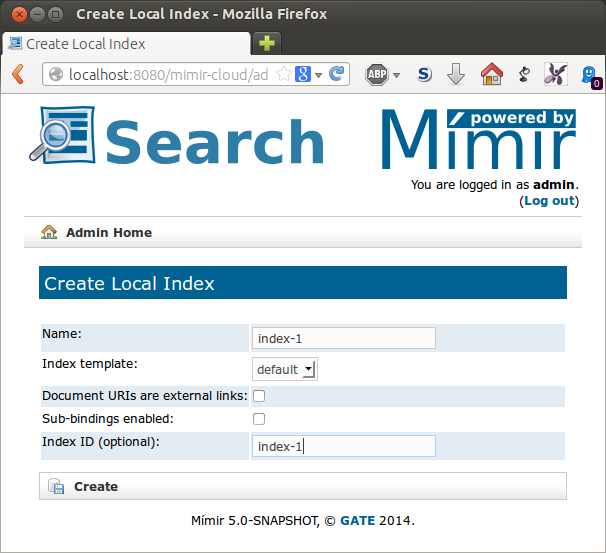
\includegraphics[scale=0.5]{img/new-local-index}
\end{center}
\caption{Creating a new local index}
\label{fig:new-local-index}
\end{figure}
%
The index will be assigned a unique identifier and a new directory will be
created under the \verb|indexBaseDirectory| you configured earlier to
hold the index data.  The newly-created index will start in the {\em ready}
state (see Figure~\ref{fig:local-index-created}), ready to receive documents
for indexing.  For details of how to submit documents to the index, see
Chapter~\ref{sec:indexing}.
%
\begin{figure}[htb!]
\begin{center}
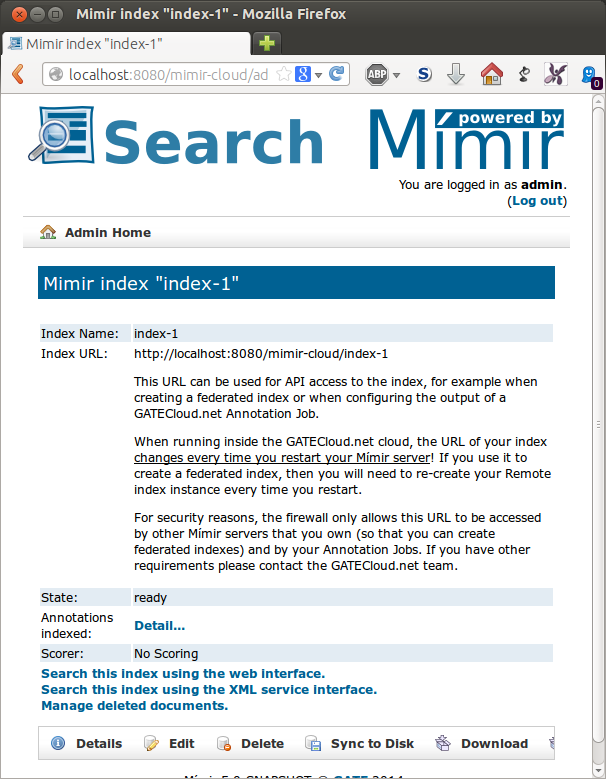
\includegraphics[scale=0.5]{img/local-index-created}
\end{center}
\caption{Results of creating a new local index}
\label{fig:local-index-created}
\end{figure}
%

This {\em index information} page can be accessed at any time by clicking the
link for the relevant index name from the \Mimir\ front page
(Figure~\ref{fig:local-index-list}).
%
\begin{figure}[htb!]
\begin{center}
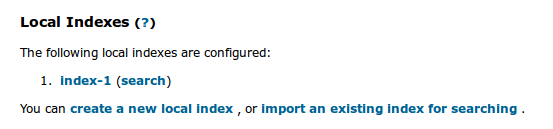
\includegraphics[scale=0.5]{img/local-index-list}
\end{center}
\caption{List of local indexes on the \Mimir\ front page}
\label{fig:local-index-list}
\end{figure}
%
At any time, the index can then be searched using the tools described in
Chapter~\ref{sec:searching}. Recently added documents only become avaialble for
searching after a {\em sync-to-disk} has taken place. Sync operations happen
automtaically at regular intervals, or can be triggered by the user by pressing
the {\em Sync to Disk} button seen at the bottom of the index information page.

\subsection{Working with Remote and Federated Indexes}

The architecture of \Mimir\ is designed to make working with remote and
federated indexes as transparent as possible.  The setup process will obviously
vary for the different index types, but once created the process of submitting
documents for indexing or of performing queries is exactly the same for all
indexes.

\subsubsection{Remote indexes}\label{sec:admin:remote-index}
A {\em remote} index is a mechanism whereby one \Mimir\ instance can
transparently index documents in, or send queries to, an index that is located
in a different \Mimir\ instance, typically running on separate hardware.  To
connect one {\em master} \Mimir\ instance to an index running in another {\em
slave} instance, first visit the index information page for the relevant
index on the slave and make a note of its {\em remote URL} (typically a URL of
the form \verb|http://server:port/mimir/remote/{UUID}|).  Now on the front page
of the master instance, select the {\em connect to a new remote index} link.
This will present a form (Figure~\ref{fig:connect-remote-index}) asking for a
name for the remote index (which need not be the same as the name of the index
on the slave), and a {\em remote URL} which is the one you made a note of from
the slave above. You should never create a remote index pointing to another
index in the same \Mimir\ instance. Such a configuration is not supported and
will lead to errors!
\begin{figure}[htb!]
\begin{center}
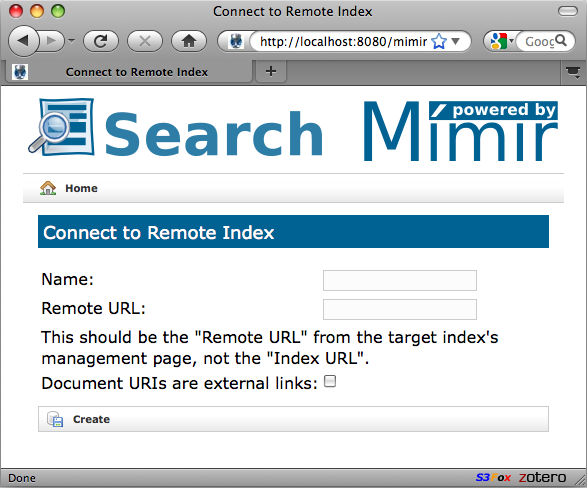
\includegraphics[scale=0.5]{img/connect-remote-index}
\end{center}
\caption{Connecting to a remote index}
\label{fig:connect-remote-index}
\end{figure}
%

The remote index defined on the master server will synchronise its state with
that of the underlying index on the slave, and once created will be usable
exactly like a local index.  However remote indexes are rarely used directly,
as in most cases it is more efficient to operate on the slave instance
itself.  The main benefit of remote indexes comes when they are used as part
of a {\em federated index}.

\subsubsection{Federated indexes}

A {\em federated index} is a device to bundle several indexes (which can
themselves be local, remote or federated) together so they can be used as a
single index.  Documents for indexing are shared out between the component
{\em sub-indexes}, and searches are performed by all sub-indexes in parallel.
Thus a federation of five indexes each containing 200,000 documents will
typically run queries faster than a single index containing 1 million
documents.  To create a federated index, go to the \Mimir\ front page and
select the {\em create a new federated index} link.  This will present a form
(Figure~\ref{fig:new-federated-index}) asking for a name for the federated
index.  The form also includes a multiple-selection list to specify the
sub-indexes to be included in the federated index.  Select the appropriate
entries from this list using the usual multiple list selection mechanism
(ctrl-click on Windows or Linux, cmd-click on Mac OS X) and press the
{\em Create} button to create the index.
%
\begin{figure}[htb!]
\begin{center}
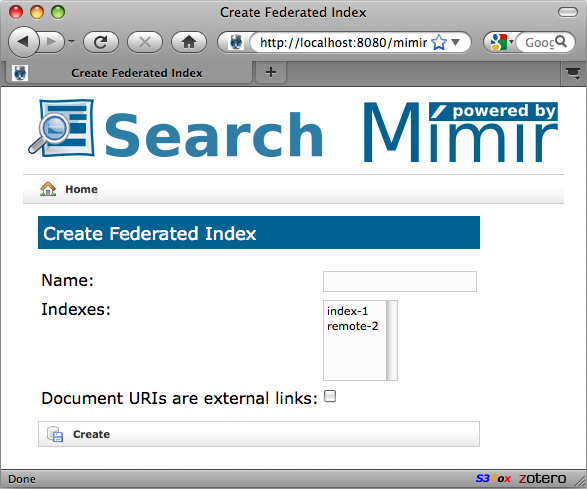
\includegraphics[scale=0.5]{img/new-federated-index}
\end{center}
\caption{Creating a new federated index}
\label{fig:new-federated-index}
\end{figure}
%
Once created the federated index will be usable exactly like a local or remote
index.

\subsection{Deleting Indexes}

If an index registered with Mimir is no longer required it can be deleted by
selecting the {\em Delete} button from the index information page (accessible by
clicking on the name of the relevant index on the \Mimir\ front page).  For
remote and federated indexes this simply deletes the ``registration'' of the
index with \Mimir, which can be easily re-created as above.  For local indexes
it also offers the option to delete the underlying index files from disk.  If a
local index is deleted without deleting the disk files then the index can be
re-created later using the {\em import an existing index for searching} option
from the \Mimir\ front page.

\Mimir\ will not allow the deletion of an index which is currently part of a
federated index in the same \Mimir\ instance.  To delete such an index, it must
first be removed from the federated index.  This guarantee only applies to
indexes within a {\em single} \Mimir\ instance --- \Mimir\ does not prevent the
deletion of an index on a slave instance which is being used as a remote index
by a master instance (it prevents the deletion of the remote index definition
in the master but not the slave index it points to).  However to do so would
put the remote index on the master (and hence any federated index that it is
part of) into the {\em failed} state, preventing further use until the problem
is resolved.

\section{``Deleting'' Documents from a \Mimir\ Index}\label{sec:admin:takedown}

While \Mimir\ indexes are not directly modifiable once they have been created,
there are situations in which it is necessary to remove documents that should
not have been indexed in the first place, or documents that may be considered
libellous, etc.  To support this, \Mimir\ provides a mechanism to mark
individual documents in the index as ``deleted'', and any documents so marked
will be excluded from future queries.  It is not possible to completely delete
the data from the index files on disk, short of completely re-building the
index from scratch, but documents marked as deleted are not accessible through
any of the public \Mimir\ APIs or user interfaces.

To mark a document as deleted (or to remove an existing deletion marker, making
the document available for queries again), use the ``Manage deleted documents''
link from the index's administration page.  This will present the screen shown
in figure~\ref{fig:deleted-documents}, with a text box into which you can type
one or more (space-separated) document IDs, and choose whether to mark them as
deleted or as ``not deleted'' (i.e. to remove any existing deletion markers for
those document IDs).
%
\begin{figure}[htb!]
\begin{center}
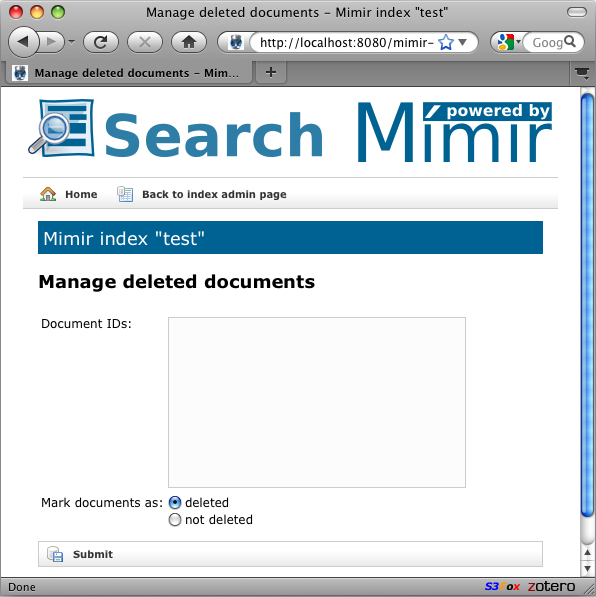
\includegraphics[scale=0.5]{img/deleted-documents}
\end{center}
\caption{Managing deleted documents}
\label{fig:deleted-documents}
\end{figure}

Note that the IDs required here are not the URIs that were provided with the
documents when they were indexed, but the internal \Mimir\ document IDs which
are numbers starting from 0, as returned in the hit lists and ``getDocumentId''
by the \Mimir\ query APIs (see section~\ref{sec:search:service}).
